\section{Implementierung}

In diesem Kapitel wird die Implementierung des Projektes mit Fokussierung auf die einzelnen Komponenten beschrieben.

\subsection{Kommunikation}

Die Kommunikation der einzelnen Komponenten des Schwarmverhaltens baut auf einer klar definierten Struktur, um ein verteiltes System zu ermöglichen, siehe Abbildung \ref{fig:full_classdiagram}. Die Daten werden dabei als \gls{json} Objekte zur optimalen plattformübergreifenden Interpretation versendet, wobei jeweils die entsprechende Bibliothek zur Serialisierung verwendet wird.
\begin{verbatim}
\end{verbatim}
\begin{figure}[h]
	\begin{center}
		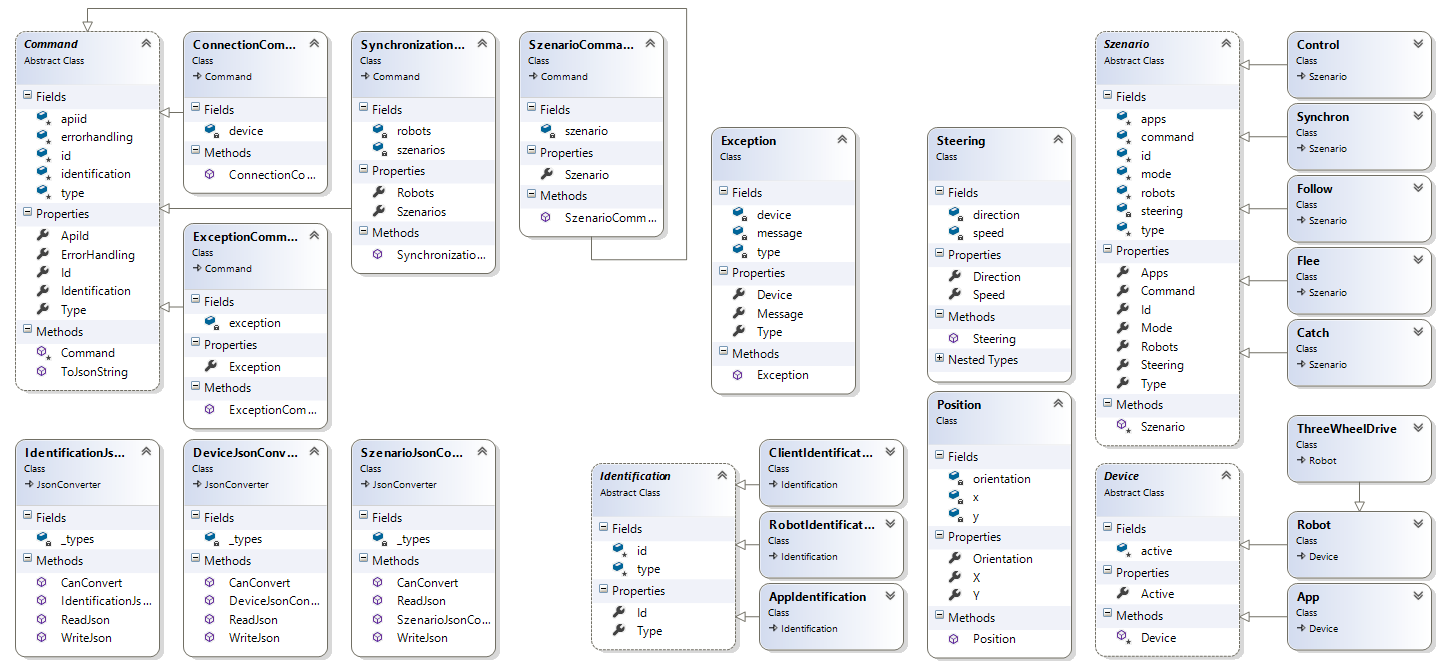
\includegraphics[width=0.95\textwidth]{images/uml/full_class_diagram.png}
	\end{center}
	\caption{Aufbau Commands}
	\label{fig:full_classdiagram}
\end{figure}

\newpage
\noindent
Der Kern zur Implementierung der Kommunikation erfolgt in zwei Methoden, die auf jeder Komponente zur Verfügung stehen. Diese dienen zum Versenden, sowie Empfangen von Daten, wobei diese als Zeichenkette serialisiert und in Bytes aufgeteilt werden, siehe Abbildung \ref{fig:SendCommand}. Um den vollständigen Umfang der Daten zu erfassen, wird die Größe ermittelt und standardmäßig mittels vier Bytes übertragen. Dadurch ist eine maximale Paketgröße von 32 Byte möglich, was einer Länge von etwa 4 Milliarden Zeichen entspricht. Die Interpretation zum Empfangen erfolgt mit ähnlichem Muster, indem zunächst die Größe der Daten festgestellt wird und die Daten deserialiert werden, siehe Abbildung \ref{fig:ReceiveCommand}.

\begin{figure}[h]
	\centering
	\subfloat[Versende Kommando]{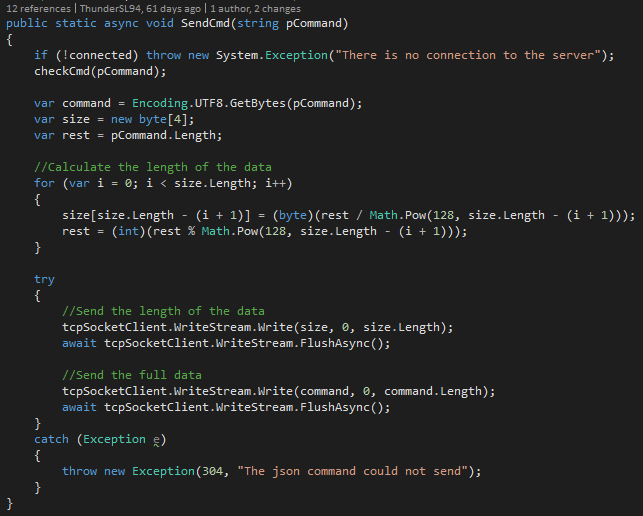
\includegraphics[width=0.6\textwidth]{images/code/SendCommand.png}\label{fig:SendCommand}}
	\qquad
	\subfloat[Empfange Kommando]{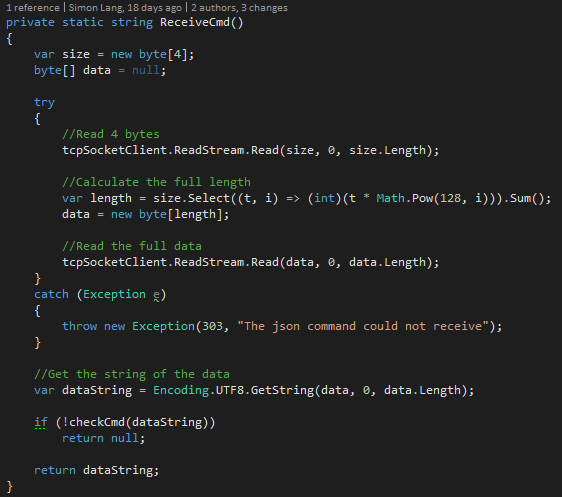
\includegraphics[width=0.6\textwidth]{images/code/ReceiveCommand.png}\label{fig:ReceiveCommand}}
	\caption{Kommunikation}
\end{figure}

\newpage
\paragraph{Kommandos}

\begin{wrapfigure}{r}{0.55\textwidth}
	\begin{center}
		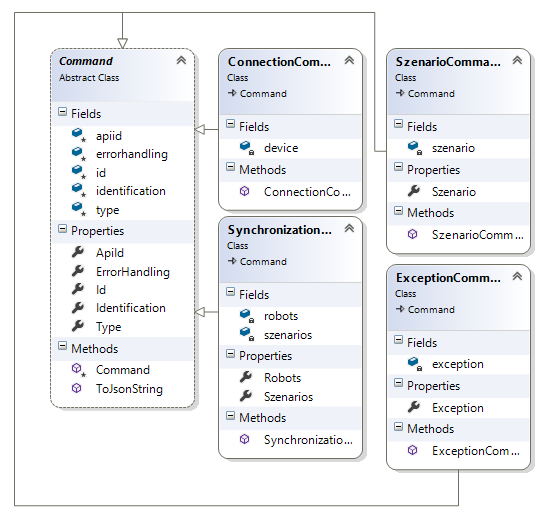
\includegraphics[width=0.5\textwidth]{images/uml/commands.png}
	\end{center}
	\caption{Kommandos}
	\label{fig:commands_classdiagram}
	\begin{center}
		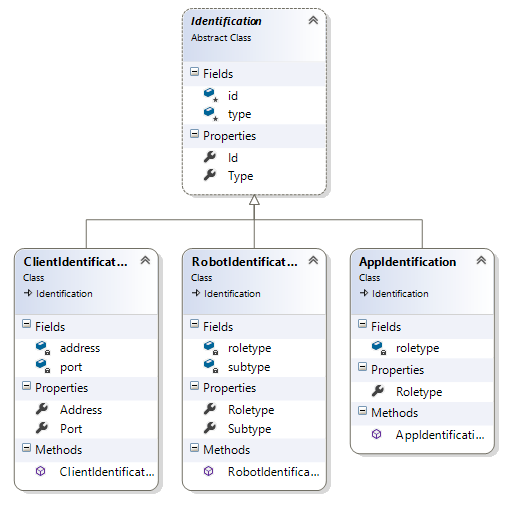
\includegraphics[width=0.5\textwidth]{images/uml/identification.png}
	\end{center}
	\caption{Identifikation}
	\label{fig:identification_classdiagram}
\end{wrapfigure}

stellen die Basis der Kommunikationsstruktur sowie den aktuellen Kontext dar, indem sich die Software befindet, siehe Abbildung \ref{fig:commands_classdiagram}. Sie enthalten grundlegende Attribute zur allgemeinen Identifikation des Kommandos, die zur Interpretation verwendet, welche über definierte Enums ausgewählt werden. Je nach Kommando sind zusätzliche Objekte enthalten, die durch die jeweilige Id vordefiniert sind.\\

\paragraph{Identifikationen}

stellt die individuelle Identität der einzelnen Komponente dar, siehe Abbildung \ref{fig:identification_classdiagram}. Diese wird durch eine fortlaufende Identifikationsnummer, Typen und je nach Ableitung weiteren Attributen erreicht. Um die jeweiligen Kommandos entsprechend zuzuordnen, sind diese in jedem Kommando vorhanden und bilden die Basisobjekte. Die unterschiedlichen Typen sind dabei für verschiedene Kontexte der Software zuständig. Die ClientIdentification stellt einerseits die Verbindung einer allgemeinen Komponente zur Desktopanwendung dar, wogegen die Robot- bzw. AppIdentification die spezifische Identifikation der Komponente darstellt. Die Erstellung der Identifikation erfolgt wiederholt zur Anmeldung der Komponente am System. Zunächst wird ein leeres Objekt erzeugt, dass anschließend durch abfragende Kommandos an die entsprechende Komponente befüllt wird, welche hinterher eine berechnete Identifikationsnummer erhält.

\newpage
\paragraph{Geräte}

\begin{wrapfigure}{r}{0.55\textwidth}
	\begin{center}
		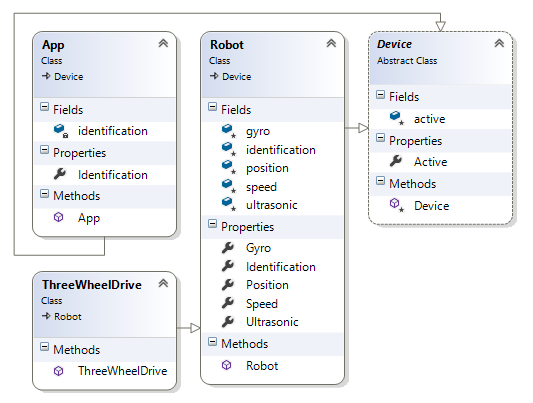
\includegraphics[width=0.5\textwidth]{images/uml/devices.png}
	\end{center}
	\caption{Devices}
	\label{fig:devices_classdiagram}
	\begin{center}
		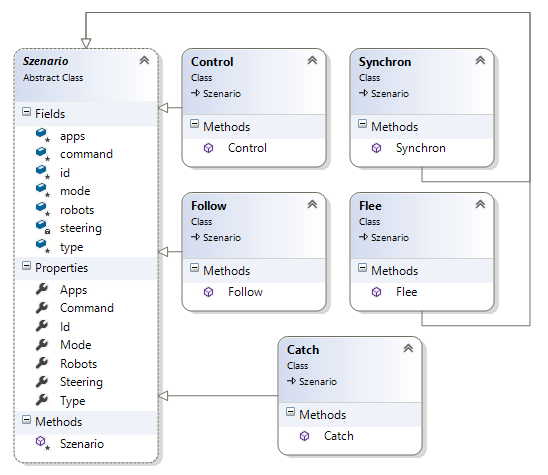
\includegraphics[width=0.5\textwidth]{images/uml/szenarios.png}
	\end{center}
	\caption{Scenarios}
	\label{fig:szenarios_classdiagram}
\end{wrapfigure}

stellen die Komponenten dar, die an einem Szenario eines Schwarmverhaltens teilnehmen, siehe Abbildung \ref{fig:devices_classdiagram}. Sie enthalten jeweils spezifische Identifikations Objekte, zur gegenseitigen Zuordnung, sowie die erfassten Daten der entsprechenden Systeme. Die Unterscheidung erfolgt in zwei Komponenten, dem Robot und der App, wobei der Roboter in die jeweiligen Untertypen gegliedert werden kann. 

\paragraph{Szenarios}

stellen den Ablauf des Schwarmverhaltens dar, in dem sich der Nutzer befindet, siehe Abbildung \ref{fig:szenarios_classdiagram}. Sie enthalten die jeweiligen Teilnehmer des Szenarios, sowie die Steuerungsinformationen und damit die gesamten Daten des aktuellen Kontextes. Diese Objekte werden laufend aktualisiert und besitzen lediglich zur Laufzeit des Szenarios ihre Gültigkeit. Dabei existieren verschiedene Kategorien von Szenarien, siehe Abschnitt \ref{szenarien}. Diese definieren jeweils einen unterschiedlichen Kontext und besitzen daher je nach Szenario zusätzliche Attribute.

\newpage
\paragraph{Konverter}

\begin{wrapfigure}{r}{0.55\textwidth}
	\begin{center}
		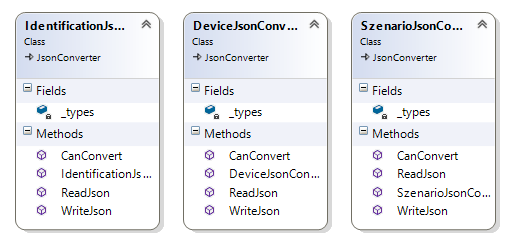
\includegraphics[width=0.5\textwidth]{images/uml/json_converter.png}
	\end{center}
	\caption{JsonConverter}
	\label{fig:converter_classdiagram}
\end{wrapfigure}

dienen der Deserialisierung von abstrakten \gls{json} Objekten, welche nicht direkt identifiziert werden können, siehe Abbildung \ref{fig:converter_classdiagram}. Dazu gehören abstrakte Klassen, sowie Schnittstellen, welche keinem spezifischen Objekt zugeordnet werden kann. Die Implementierung erfolgt durch die Überschreibung der entsprechenden Methoden zur Deserialisierung und Serialisierung, siehe Abbildung \ref{fig:ConverterRead} und \ref{fig:ConverterWrite}. Je nach Anwendung, wird ein Parameter übergeben, der das Objekt als Zeichenkette beinhaltet. Dieses wird durch eine Abfolge von Bedingungen auf den Typen geprüft wird, um das Objekt zu erstellen.\\

\begin{figure}[h]
	\centering
	\subfloat[ReadJson]{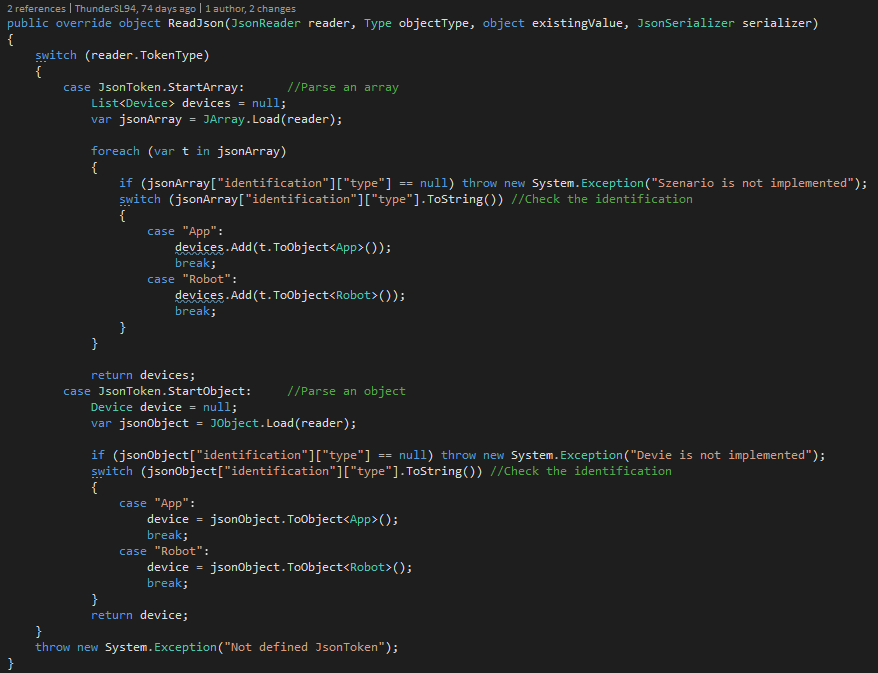
\includegraphics[width=0.6\textwidth]{images/code/DeviceConverterRead.png}\label{fig:ConverterRead}}
	\qquad
	\subfloat[WriteJson]{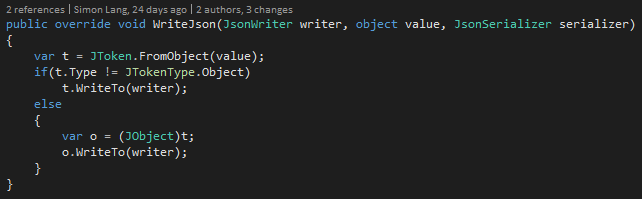
\includegraphics[width=0.6\textwidth]{images/code/DeviceConverterWrite.png}\label{fig:ConverterWrite}}
	\caption{Device JsonConverter}
\end{figure}

\newpage
\subsection{\gls{app}}

Die Erstellung der App erfolgt in einer plattformübergreifenden Implementierung durch Xamarin in C\#. Kernelemente stellen hierbei die Struktur, Oberfläche, Businesslogik sowie das Kommunikationssystem dar.
Diese gliedern sich in zwei Projekte, der \gls{app} sowie das Kommunikationssystem mit seinen Strukturen, welches eine Bibliothek als \acrshort{pcl} bildet, wie sie in anderen Komponenten von Xamarin zu finden sind. Somit lässt sich die Logik einmalig implementieren und kann auf andere Systemen entsprechend übertragen werden.\\
Die \gls{app} besteht dabei aus einer \acrshort{pcl}, welche die jeweiligen Plattformen je nach eingestelltem System einbindet und einen plattformspezifischen Quellcode als \gls{il} erzeugt. Der plattformübergreifende Quellcode kann dabei in der \acrshort{pcl} implementiert werden, wobei plattformspezifische Anpassungen über die entsprechenden Projekte vorgenommen werden können.

%Screenshot visual studio

\subsubsection{Workflow} %Struktur

Die Struktur der \gls{app} basiert auf dem in Xamarin weit verbreiteten Design Pattern \acrlong{mvvm}, welches durch ein Benachrichtigungssystem eine Abspaltung der Daten, \gls{gui} und dem Businesscode erlaubt. Die einzelnen Seiten der App sind code behind, indem zunächst die Page dargestellt ist, indem diese durch xaml designd wird und dahinter die entsprechende Klasse mit dem dazugehörigen businesscode abgelegt ist.

\paragraph{\acrfull{mvvm}}

stellt ein Design Pattern dar, welches eine grundlegende Struktur im Quellcode ermöglicht. Dabei wird die erstellte Benutzeroberfläche von der Logik, sowie den Daten getrennt, um Änderungen unabhängig voneinander durchführen zu können. Um die Teile des Quellcodes zu verbinden wird auf Bindings gesetzt, die dafür zuständig sind, die jeweiligen Objekte gegenseitig zu aktualisieren.

\begin{figure}[h]
	\begin{center}
		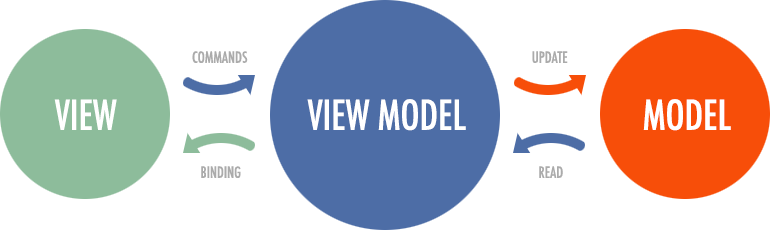
\includegraphics[width=0.95\textwidth]{images/implementation/mvvm.png}
		\caption{\acrlong{mvvm} \cite{Brecht.MVVMEntity}}
	\end{center}
	
	\label{fig:mvvm}
\end{figure}

\paragraph{Bindings}

sind für die gegenseitige aktualisierung von Daten der jeweiligen Objekte zuständig. SIe entsprechen ihrem Sinn nach dem Observer Design Pattern und knüpfen an die VIewModels des MVVM an, wobei die dort definierten Objekte mit die der gleichnamigen View und den MOdel Objekten verbunden sind. Durch eine aktualisierung der Daten werden dabei die jeweilig verbundennen aktualisiert. DIes kann auf zwei verschiedenen wegen von statten gehen. Manuell, durch das aufrufen der entsprechenden Methode im ViewModel, andererseits automatisch, durch Attribute, wobei bei einer Änderung, die Methode automatisch angestoßen wird.

% Observer Pattern

\subsubsection{\acrfull{gui}} %Oberfläche

Die Oberfläche der \gls{app} wird mittels XAML erstellt, welche auf der Basis von XML ist. Dabei werden die einzelnen ELemente untereinnander Strukturuert, wobei der ENtwickler in Xamarin verschiedene Möglichkeiten des Designs besitzt. Grundlegend ist die entscheidung, ob eine plattformspezifisches Design sinnn macht, oder aber ein plattformübergreifendes, wobei dieses weniger Freiheiten bietet. Die plattformübergreifendes Design besitzt eine Reihe von grundlegeneden Layouts, die für Xamamrin eingesetzt werden können, sowie unterschiedliche Seitenarten. Views
Seiten (ContentPage, MasterDetailPage, NavigationPage, TabbedPage, TemplatedPage, CaruselPage)
View (ContentPresenter, ContentVIew, ScrollVIew, Frame, TemplatedVIew)
Layout (Stacklayout, absolutLayout, RelativeLayout, GridLayout)

Weitere standardelemente

Durch verschiednene Packages könenn dabei viele Zusätzliche DInge erstellt werden

%General, XAML stuff

\paragraph{LogIn Page}

\paragraph{Home Page}

\paragraph{Option Page}

\paragraph{List Page}

\paragraph{Szenario Page}

\subsubsection{Buisnesslogic} %Logik

\subsubsection{Deployment}

\subsection{Backend}

\begin{comment}
Aufbau
Interpreter
Mechanismen
GUI
\end{comment}

\subsection{Robot}

\begin{comment}
Aufbau
Robot
RobotController
EV3 Library
GUI
\end{comment}